% Blocking the First Connection -- draft for internal review.
% Build:  cd paper && latexmk -pdf main.tex
\documentclass[sigconf,nonacm]{acmart}

\usepackage{tikz}
\usetikzlibrary{arrows.meta,positioning,fit,backgrounds}
\usepackage{booktabs}
\usepackage{siunitx}
\sisetup{group-separator={,},group-minimum-digits=4}

\settopmatter{printacmref=false, printfolios=true}
\setlength{\emergencystretch}{1.5em}
\renewcommand\footnotetextcopyrightpermission[1]{}
\pagestyle{plain}

\newcommand{\sys}{DPI Guard}
\newcommand{\todo}[1]{\textcolor{red}{[TODO: #1]}}

\begin{document}

\title{Blocking the First Connection: Where the Time Goes in DPI-Guided XDP Enforcement}
\subtitle{Draft for internal review}

\author{Shelender Kumar}
\affiliation{%
  \institution{School of Electrical Engineering and Computer Science (SEECS), NUST}
  \city{Islamabad}
  \country{Pakistan}}

\begin{abstract}
Gateways that block domains must turn names seen by deep packet inspection (DPI) into packet
drops on IP addresses. We ask how long that takes and whether the first connection to a blocked
domain gets through. We built \sys{}, which couples NFStream/nDPI flow inspection with an
eBPF/XDP blocklist, and measured three decision strategies on a Linux testbed. Acting when a
flow is exported blocked domains a median of \SI{5.8}{\second} after the ClientHello and never
stopped the first connection; on a quiet link, 11 of 30 flows were never acted on. Acting on
every packet inside the DPI engine cut the median to \SI{489}{\milli\second}, a delay we trace to
buffered packet capture rather than to classification. A fast path that parses only TLS
ClientHellos from an unbuffered, BPF-filtered socket blocked domains \SI{0.81}{\milli\second}
after the ClientHello and stopped 30 of 30 first connections. The XDP hash-map blocklist kept a
constant per-packet cost from 1 to \num{10000} entries, while linear iptables rules lost 98\% of
their throughput. We release the system, the testbed and all raw measurements.
\end{abstract}

\keywords{eBPF, XDP, deep packet inspection, TLS SNI, packet filtering, measurement}

\maketitle

%% ---------------------------------------------------------------------------------------
\section{Introduction}

Network operators block domains, but packets carry IP addresses. A campus, enterprise or home
gateway that must stop traffic to \texttt{youtube.com} has to learn which server addresses
currently serve that name, and then drop their packets fast enough for the policy to hold.

Deep packet inspection solves the first half: libraries such as nDPI~\cite{ndpi} read the
server name from the TLS ClientHello's Server Name Indication (SNI)~\cite{rfc6066,rfc8446},
from QUIC~\cite{rfc9000}, DNS or the HTTP \texttt{Host} header. eBPF and the eXpress Data Path
(XDP)~\cite{xdp} solve the second: an XDP program drops packets in the driver, before the kernel
allocates socket buffers, and its blocklist can be changed at run time through BPF maps.

This paper studies what happens \emph{between} the two halves: how long it takes from the
moment a blocked name appears on the wire until the kernel drops that server's packets, and
whether the first connection completes in the meantime. A blocker that lets every first
connection through is weak in practice: a page load, an API call or a software update may need
only one connection.

We built \sys{}, an open-source DPI-guided XDP blocker~\cite{dpiguard}, and measured three
decision strategies. Our main finding is that the dominant delay is neither DPI nor the kernel,
but how packets reach user space:
\begin{itemize}
  \item Acting when a flow is \emph{exported} waits for the flow's idle timeout, so the first
        connection always completes (median time-to-block \SI{5.8}{\second}); on a quiet link
        the flow may never be exported.
  \item Acting in a \emph{per-packet} DPI hook is faster, but buffered libpcap capture delivers
        packets in blocks on a timer, adding a uniform 0--\SI{1}{\second} delay (median
        \SI{489}{\milli\second}).
  \item A \emph{fast path}, a filtered \texttt{AF\_PACKET} socket that wakes only for TLS
        ClientHellos, reduces time-to-block to \SI{0.81}{\milli\second}; the server's first
        reply is dropped and every first connection fails.
\end{itemize}

\noindent\textbf{Contributions.} (1)~The design and implementation of a DPI-guided XDP domain
blocker with a two-path architecture and a header-free user-space controller that drives BPF
maps through the \texttt{bpf(2)} system call (\S\ref{sec:design}). (2)~A measurement of
time-to-block for three decision strategies that identifies capture buffering as the dominant
delay (\S\ref{sec:ttb}). (3)~A comparison of drop cost and blocklist scaling for XDP hash maps,
nftables sets and iptables rules (\S\ref{sec:cost}). (4)~A policy model that maps domain rules
to IP addresses with exact unblocking and reports collateral blocking (\S\ref{sec:design}).

%% ---------------------------------------------------------------------------------------
\section{Background and Related Work}
\label{sec:background}

\textbf{Packet capture.} User-space monitors read packets through libpcap, which descends from
the BSD Packet Filter~\cite{bpf}. On Linux, libpcap uses a memory-mapped \texttt{TPACKET\_V3}
ring that hands \emph{blocks} of packets to user space when a block fills or its timeout
expires, trading latency for throughput. Immediate mode~\cite{pcapimmediate} removes this delay,
but frameworks built on libpcap do not always expose it.

\textbf{DPI and flow export.} nDPI~\cite{ndpi} classifies flows and extracts metadata such as
the TLS server name. NFStream~\cite{nfstream} wraps nDPI in a Python flow-measurement framework
that exports a record when a flow ends (idle or active timeout) and runs user plugins on every
packet.

\textbf{Kernel packet filtering.} XDP~\cite{xdp} runs verified eBPF programs at the earliest
point of the receive path and is used in production for DDoS mitigation~\cite{bertin}. Scholz et
al.~\cite{scholz} analysed the performance of eBPF-based filtering, and bpf-iptables~\cite{bpfiptables}
showed that rule-by-rule iptables matching degrades with the number of rules while eBPF data
structures do not. nftables sets offer hash-based matching inside netfilter, including on the
early \texttt{netdev} ingress hook.

\textbf{Name-based blocking and its limits.} SNI is sent in clear text in TLS 1.2 and
1.3~\cite{rfc6066,rfc8446}, which makes it a common signal for filtering and
censorship~\cite{chai}; Encrypted Client Hello (ECH)~\cite{ech} hides it. Blocking by IP has
collateral effects when domains share addresses, and Hoang et al.~\cite{hoang} show how widely
domains are co-hosted.

\textbf{Gap.} Prior work evaluates either classification or filtering throughput in isolation.
We measure the end-to-end delay between classification and enforcement, and whether a
DPI-guided blocker stops the \emph{first} connection.

%% ---------------------------------------------------------------------------------------
\section{Design}
\label{sec:design}

\sys{} splits the work in two: user space decides \emph{which} addresses to block from the
names it observes, and an XDP program in the kernel drops their packets
(Figure~\ref{fig:arch}).

\begin{figure}[t]
\centering
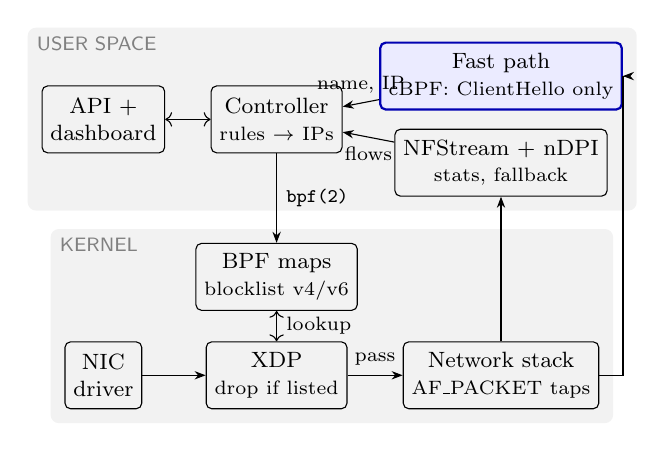
\begin{tikzpicture}[
  font=\footnotesize,
  box/.style={draw, rounded corners=2pt, align=center, minimum height=0.85cm, inner sep=3pt},
  hl/.style={box, draw=blue!70!black, fill=blue!8, line width=0.8pt},
  arr/.style={-{Stealth[length=4pt]}, thin},
  lane/.style={draw=none, fill=gray!10, rounded corners=3pt, inner sep=5pt}]
  % user space
  \node[hl]  (fast) at (5.6, 2.55) {Fast path\\{\scriptsize cBPF: ClientHello only}};
  \node[box] (nf)   at (5.6, 1.45) {NFStream + nDPI\\{\scriptsize stats, fallback}};
  \node[box] (ctl)  at (2.75, 2.0) {Controller\\{\scriptsize rules $\rightarrow$ IPs}};
  \node[box] (ui)   at (0.55, 2.0) {API +\\dashboard};
  % kernel
  \node[box] (maps) at (2.75, 0.0) {BPF maps\\{\scriptsize blocklist v4/v6}};
  \node[box] (nic)  at (0.55, -1.25) {NIC\\driver};
  \node[box] (xdp)  at (2.75, -1.25) {XDP\\{\scriptsize drop if listed}};
  \node[box] (stk)  at (5.6, -1.25) {Network stack\\{\scriptsize AF\_PACKET taps}};
  \begin{scope}[on background layer]
    \node[lane, fit=(fast)(nf)(ctl)(ui)] (us) {};
    \node[lane, fit=(maps)(nic)(xdp)(stk)] (ks) {};
  \end{scope}
  \node[anchor=north west, font=\scriptsize\sffamily, gray] at (us.north west) {USER SPACE};
  \node[anchor=north west, font=\scriptsize\sffamily, gray] at (ks.north west) {KERNEL};
  \draw[arr] (nic) -- (xdp);
  \draw[arr] (xdp) -- node[above, font=\scriptsize] {pass} (stk);
  \draw[arr, <->] (xdp) -- node[right, font=\scriptsize] {lookup} (maps);
  \draw[arr] (ctl) -- node[right, font=\scriptsize] {\texttt{bpf(2)}} (maps);
  \draw[arr] (stk.north) -- ++(0,0.35) -| (nf.south);
  \draw[arr] (fast) -- node[above, font=\scriptsize] {name, IP} (ctl);
  \draw[arr] (nf) -- node[below, font=\scriptsize] {flows} (ctl);
  \draw[arr, <->] (ui) -- (ctl);
  \draw[arr] (stk.east) -- ++(0.3,0) |- (fast.east);
\end{tikzpicture}
\caption{\sys{} architecture. Two taps observe server names; the controller turns domain rules
into IP addresses and writes them to pinned BPF maps that the XDP program consults.}
\label{fig:arch}
\end{figure}

\textbf{Enforcement.} One XDP program on the monitored interface parses Ethernet, up to two
VLAN tags and the IPv4 or IPv6 header, and looks up both the source and destination address in
a hash map with \num{65536} entries per address family. A hit returns \texttt{XDP\_DROP} and
increments that entry's packet and byte counters; a miss returns \texttt{XDP\_PASS}. Matching
both directions drops a blocked server's replies on an end host and outbound requests on a
gateway. Global counters live in a per-CPU array, so the hot path takes no shared locks.

\textbf{Decision.} Two taps feed the controller. The \emph{fast path} is an \texttt{AF\_PACKET}
socket with a 28-instruction classic-BPF filter that accepts only IPv4 TCP segments to port 443
whose payload begins with a TLS handshake record of type ClientHello; user space therefore
wakes only for connection openings, parses the SNI and reports (name, server IP) at once.
\emph{NFStream with nDPI} inspects all traffic, keeps per-domain statistics, and acts as a
fallback for names the fast path cannot see (QUIC, DNS, HTTP, a ClientHello split across
segments).

\textbf{Policy.} A rule such as \texttt{youtube.com} matches the name and all subdomains; the
most specific rule wins. The controller remembers every observed (domain, IP) pair, so adding a
rule blocks already-seen addresses at once, and removing one unblocks exactly the addresses no
remaining rule needs. When a blocked address also serves an allowed name, the controller
reports it as collateral.

\textbf{Implementation.} \sys{} is about \num{1000} lines of Python plus a 128-line XDP program
compiled ahead of time with clang and loaded with iproute2. The controller manipulates the
pinned maps with five \texttt{bpf(2)} commands issued through \texttt{ctypes}, so it needs no
BCC or kernel headers at run time. A Flask API exposes rules and counters. Twenty-six
automated tests, three of which run XDP and nftables on a veth pair inside a network namespace,
check enforcement end to end.

%% ---------------------------------------------------------------------------------------
\section{Methodology}
\label{sec:method}

\textbf{Testbed.} A KVM virtual machine with 4~vCPUs (Intel Xeon, \SI{2.8}{\giga\hertz}),
\SI{15}{\giga\byte} RAM, Linux 6.18 and iptables 1.8.10 (nf\_tables back end). A sender in a
network namespace reaches the host through a veth pair; filters attach to the host-side
interface (XDP in native mode). A TLS~1.3 server in the namespace answers one HTTP request per
connection.

\textbf{Time-to-block (\S\ref{sec:ttb}).} For each decision mode we run 30 trials. Trial $i$
connects to its own server address with SNI \texttt{t$i$.blocked.test}, so earlier blocks never
affect later trials. The client records the time just before sending its ClientHello; \sys{}
records when it wrote the IP to the XDP map. Their difference is the \emph{time-to-block}.
Every trial is paired with a control connection to an allowed name on another address, which
must succeed.

\textbf{Drop cost and scaling (\S\ref{sec:cost}).} A C sender (\texttt{sendmmsg}, batches of 64
UDP packets, 64-byte frames) floods the host for \SI{5}{\second} while pinned to one vCPU. On a
veth pair the receive path runs on the sending CPU, so the achieved sender rate measures the
whole per-packet path. For drop cost we block the sender's address; for scaling we fill the
blocklist with $N$ random addresses that never match, so every packet takes the full
no-match path. Each configuration runs 5 times; we report the mean and sample standard
deviation.

%% ---------------------------------------------------------------------------------------
\section{Results}

\subsection{Time-to-Block}
\label{sec:ttb}

\begin{figure}[t]
  \centering
  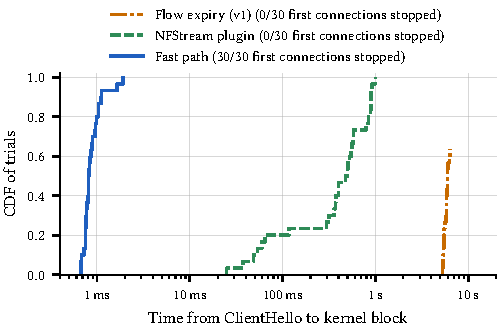
\includegraphics[width=\columnwidth]{figures/time_to_block.pdf}
  \caption{Time from the client's ClientHello to the kernel block, 30 trials per mode. The
  expiry curve stops at 19/30: the remaining flows were never exported.}
  \label{fig:ttb}
\end{figure}

Figure~\ref{fig:ttb} shows the distribution of time-to-block for each mode.

\textbf{Flow expiry} acts only after the connection has ended and stayed idle for the
\SI{5}{\second} timeout. Every first connection completed, and the block landed
5.3--\SI{6.3}{\second} after the ClientHello. NFStream checks for idle flows only when new
packets arrive: the last 11 trials, after which the link went quiet, were never enforced during
the \SI{9}{\second} observation window. On a quiet link, export-based enforcement has no upper
bound.

\textbf{The NFStream plugin} sees the server name on the connection's fourth packet, yet the
block landed 25--\SI{999}{\milli\second} after the ClientHello (median \SI{489}{\milli\second}).
Almost all of this delay lies between a packet's capture timestamp and the plugin call, and it
is spread evenly over 0--\SI{1}{\second}: the signature of a capture buffer released on a
timer. Classification and the map update take well under a millisecond.

\textbf{The fast path} removes the buffer: the block landed 0.67--\SI{1.91}{\milli\second}
after the ClientHello (median \SI{0.81}{\milli\second}; \SI{0.27}{\milli\second} from frame
arrival to map update). The server's first reply was dropped, so all 30 first connections
failed. All 90 control connections succeeded.

On our testbed the server answers in well under a millisecond, so even a \SI{25}{\milli\second}
block arrives too late for the plugin. Over the Internet, round-trip times of tens of
milliseconds give the fast path a wide margin, while the plugin stops a first connection only
when its 0--\SI{1}{\second} delay happens to be shorter than the RTT.
\todo{Repeat with emulated server delays of 5--\SI{100}{\milli\second} and plot the fraction of
first connections stopped against RTT.}

\subsection{Drop Cost and Blocklist Scaling}
\label{sec:cost}

\begin{table}[t]
  \caption{Sender rate with the sender's own address blocked (kpps, 5 runs).}
  \label{tab:drop}
  \small
  \begin{tabular}{@{}lrr@{}}
    \toprule
    Path & Mean & SD \\
    \midrule
    \csname @@input\endcsname figures/drop_table.tex
    \bottomrule
  \end{tabular}
\end{table}

\textbf{Drop cost.} Table~\ref{tab:drop}: dropping is cheaper than delivering, and on veth XDP
and the nftables \texttt{netdev} ingress hook perform the same within noise, both about 16\%
faster than an iptables \texttt{INPUT} rule, which runs later in the stack. We expected XDP to
lead, but on veth the sender has already allocated the socket buffer that XDP normally avoids,
and attaching XDP adds a NAPI hand-off. This result shows that the XDP enforcer costs no more
than the best netfilter alternative here; its advantage on physical NICs~\cite{xdp,scholz}
remains to be measured on our hardware.

\begin{figure}[t]
  \centering
  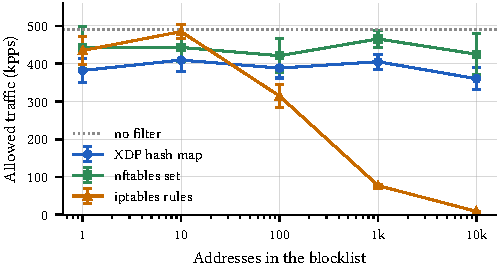
\includegraphics[width=\columnwidth]{figures/scaling.pdf}
  \caption{Allowed traffic forwarded while $N$ non-matching addresses are blocked (mean
  $\pm$ SD, 5 runs).}
  \label{fig:scaling}
\end{figure}

\textbf{Scaling.} Figure~\ref{fig:scaling}: with hash-based lookups the blocklist size does not
matter; XDP's map and the nftables set forward allowed traffic at the same rate with 1 or
\num{10000} entries. iptables evaluates its rules one by one, so every allowed packet pays for
every rule: at \num{10000} addresses it forwards \SI{8.6}{kpps}, 2\% of its single-rule rate,
consistent with the linear degradation reported for iptables~\cite{bpfiptables}. Attaching XDP
to a veth interface costs about 20\% of forwarding rate even when nothing is dropped, because
veth then processes frames through an extra NAPI step; this overhead is specific to veth.

%% ---------------------------------------------------------------------------------------
\section{Discussion}
\label{sec:discussion}

\textbf{Where the time goes.} In a DPI-guided blocker, the kernel and the classifier are fast;
the delay comes from how packets reach the classifier. Export-on-expiry ties enforcement to the
flow's end and to later traffic. A per-packet hook fixes the first problem but inherits the
capture library's buffering. A narrow, unbuffered tap for the one message that names the server
fixes both. Latency-critical decisions in monitoring systems need their own capture path.

\textbf{An operational lesson.} NFStream's meter processes ignore \texttt{SIGTERM}. When our
controller exited, they survived as orphans that kept capturing. While they ran, packets from
blocked addresses intermittently bypassed the native-mode XDP program on our veth testbed and
0/30 first connections were stopped; after the controller force-killed its children, 30/30 were
stopped. We have not determined the kernel mechanism; capture processes must be supervised as
strictly as the filter itself.

\textbf{Limitations.} \emph{Collateral blocking:} enforcement is per address, so an allowed
name sharing a CDN address with a blocked one is blocked too; \sys{} reports but cannot avoid
this~\cite{hoang}. \emph{Hidden names:} ECH~\cite{ech} hides the SNI and encrypted DNS hides
the query. \emph{Large ClientHellos:} post-quantum hybrid key shares can push the ClientHello
past one TCP segment; the fast path parses only the first segment and falls back to NFStream
otherwise. \emph{QUIC:} the fast path handles TCP only; QUIC Initial packets are encrypted with
keys derived from public values, so a QUIC fast path is feasible but not yet built.

\textbf{Threats to validity.} All measurements come from one virtual machine on a veth pair
with sub-millisecond RTT, which hides XDP's main advantage and adds a NAPI step of its own. IPv6
was disabled in the kernel, so only IPv4 was measured. Client and controller timestamps share
one clock. Samples are 30 trials per time-to-block mode and 5 runs per throughput point.

%% ---------------------------------------------------------------------------------------
\section{Conclusion}

A DPI-guided blocker is only as fast as the path that carries packets to its classifier.
Acting on exported flows took \SI{5.8}{\second} and never stopped a first connection; acting
inside the DPI engine took \SI{489}{\milli\second} because of capture buffering; a ClientHello
fast path took \SI{0.81}{\milli\second} and stopped all first connections, while the XDP
blocklist kept a constant cost from 1 to \num{10000} entries. Future work: bare-metal runs with
native-XDP NICs, collateral measurements on real CDN-hosted domains, a QUIC fast path, and
connection-level enforcement to avoid collateral blocking. Code, testbed and data are
available~\cite{dpiguard}.

\bibliographystyle{ACM-Reference-Format}
\bibliography{refs}

\end{document}
